\documentclass[11pt,a4paper]{article}
\usepackage[margin=18mm,top=22mm,bottom=20mm]{geometry}
\usepackage{fontspec}\setmainfont{Latin Modern Roman}
\usepackage{xcolor}\usepackage{amsmath,amssymb,tikz,graphicx,fancyhdr,array,needspace}
\usetikzlibrary{patterns,arrows.meta,decorations.pathmorphing,calc}
\setlength{\headheight}{14pt}
\usetikzlibrary{arrows.meta}
\pagestyle{fancy}\fancyhf{}\renewcommand{\headrulewidth}{0.4pt}
\fancyhead[L]{\textbf{M-08}}\fancyhead[C]{\itshape Fizika — yechimlar (OliyFizika.uz)}\fancyhead[R]{\textbf{Mock №8}}
\fancyfoot[C]{\thepage}
\setlength{\parindent}{0pt}\setlength{\parskip}{3pt}
\newcommand{\opt}[2]{\hspace*{4mm}#1)\ #2\par}
\newcommand{\blank}{\rule{5cm}{0.4pt}}
\begin{document}

\begin{center}{\Large\textbf{FIZIKA — YECHIMLAR}}\\[2pt]{\large Mock №8}\end{center}
\Needspace{10\baselineskip}\noindent\begin{minipage}{\linewidth}
\textbf{1.}\ Jism oltinçi sekundda 4 m yurib töxtadi. Uning ikkinçi sekunddagi yurgan masofasini (m) aniqlang.\par\smallskip
\opt{A}{18}
\opt{B}{36}
\opt{C}{24}
\opt{D}{42}
\end{minipage}\vspace{2pt}\par
\noindent\colorbox{gray!12}{\parbox{\dimexpr\linewidth-2\fboxsep}{\textbf{Javob: B) 36}}}\par\smallskip
\noindent\textit{Yechim.}\ Teskari qarab: oxirgi sekunddagi yöl $a/2=4$, $a=8$ m/s$^2$. Harakat 6 s davom etgan, $v_0=at=48$ m/s. Ikkinçi sekunddagi yöl\par
\[s_2=v_0-a\left(2-\frac12\right)=48-12=36\ \text{m}.\]\par\medskip\hrule\medskip
\Needspace{10\baselineskip}\noindent\begin{minipage}{\linewidth}
\textbf{2.}\ Idişning ostidagi yuzasi 1 cm$^{2}$ bölgan teşikdan moy oqib çiqmoqda, tezligi 1 m/s. Teşikdan 20 cm pastda moy oqimining kesim yuzasi (cm$^{2}$) qanday? $g$=10 m/s$^{2}$\par\smallskip
\opt{A}{$1/\sqrt{5}$}
\opt{B}{$1/\sqrt{17}$}
\opt{C}{$1/\sqrt{21}$}
\opt{D}{1/2}
\end{minipage}\vspace{2pt}\par
\noindent\colorbox{gray!12}{\parbox{\dimexpr\linewidth-2\fboxsep}{\textbf{Javob: A) $1/\sqrt{5}$}}}\par\smallskip
\noindent\textit{Yechim.}\ Teşikdan 20 cm pastda tezlik $v^2=v_0^2+2gh=1+4=5$, $v=\sqrt5$ m/s. Uzluksizlik tenglamasi $S_0v_0=Sv$:\par
\[S=\frac{S_0v_0}{v}=\frac{1\cdot1}{\sqrt5}=\frac{1}{\sqrt5}\ \text{cm}^2.\]\par\medskip\hrule\medskip
\Needspace{10\baselineskip}\noindent\begin{minipage}{\linewidth}
\textbf{3.}\ Radiuslari 6 cm va 4 cm bölgan şarlarning massalari mos ravişda 40 kg va 24 kg ga teng. Ular özaro 14 cm uzunlikdagi sterjen orqali boğlangan. Sistemaning massa markazi 6 cm radiusli şarning massa markazidan qanday masofada (cm) turibdi?\par\smallskip
\opt{A}{9}
\opt{B}{6}
\opt{C}{12}
\opt{D}{15}
\end{minipage}\vspace{2pt}\par
\noindent\colorbox{gray!12}{\parbox{\dimexpr\linewidth-2\fboxsep}{\textbf{Javob: A) 9}}}\par\smallskip
\noindent\textit{Yechim.}\ Şarlar markazlari orasidagi masofa $6+14+4=24$ cm. Massa markazi katta şar markazidan\par
\[x=\frac{m_2\cdot24}{m_1+m_2}=\frac{24\cdot24}{64}=9\ \text{cm}.\]\par\medskip\hrule\medskip
\Needspace{10\baselineskip}\noindent\begin{minipage}{\linewidth}
\textbf{4.}\ Tebraniş davri 0,04 s bölgan jism 10 s da neça marta tebranadi?\par\smallskip
\opt{A}{25}
\opt{B}{250}
\opt{C}{500}
\opt{D}{50}
\end{minipage}\vspace{2pt}\par
\noindent\colorbox{gray!12}{\parbox{\dimexpr\linewidth-2\fboxsep}{\textbf{Javob: B) 250}}}\par\smallskip
\noindent\textit{Yechim.}\ $N=t/T=10/0{,}04=250$.\par\par\medskip\hrule\medskip
\Needspace{10\baselineskip}\noindent\begin{minipage}{\linewidth}
\textbf{5.}\ Radiusi 1 cm bölgan temir şarni radiusi 3 cm ga yetgunça oltin ($\rho_{oltin}$ = 19300 kg/m$^{3}$) bilan qoplandi. Bu jarayonga qança (kg) oltin sarflanganini aniqlang. $\pi$ = 3\par\smallskip
\opt{A}{0,62}
\opt{B}{2}
\opt{C}{1,54}
\opt{D}{1}
\end{minipage}\vspace{2pt}\par
\noindent\colorbox{gray!12}{\parbox{\dimexpr\linewidth-2\fboxsep}{\textbf{Javob: B) 2}}}\par\smallskip
\noindent\textit{Yechim.}\ Oltin qatlam hajmi\par
\[V=\frac43\pi\left(R^3-r^3\right)=\frac43\cdot3\cdot(27-1)\cdot10^{-6}=1{,}04\cdot10^{-4}\ \text{m}^3,\qquad m=\rho V=19300\cdot1{,}04\cdot10^{-4}\approx2\ \text{kg}.\]\par\medskip\hrule\medskip
\Needspace{10\baselineskip}\noindent\begin{minipage}{\linewidth}
\textbf{6.}\ Yerda yotgan 1 kg massali jismni bikrligi 10 N/m bölgan prujina yordamida 1 m balandlikka kötarişda umumiy qanday iş bajariş kerak (J)? g=10 N/kg.\par\smallskip
\opt{A}{15}
\opt{B}{10}
\opt{C}{5}
\opt{D}{20}
\end{minipage}\vspace{2pt}\par
\noindent\colorbox{gray!12}{\parbox{\dimexpr\linewidth-2\fboxsep}{\textbf{Javob: A) 15}}}\par\smallskip
\noindent\textit{Yechim.}\ Avval prujina $x=mg/k=1$ m ga çözilib jismni yerdan uzadi (prujina energiyasi $kx^2/2=5$ J), söng jism 1 m ga kötariladi ($mgh=10$ J). Umumiy iş $15$ J.\par\par\medskip\hrule\medskip
\Needspace{10\baselineskip}\noindent\begin{minipage}{\linewidth}
\textbf{7.}\ Massasi 1,2 kg bölgan jism gorizontal tekislikda tekislikka parallel bölgan 56 N kuç bilan tortilmoqda. Jism va sirt orasidagi işqalaniş kuçini (N) toping. $\mu$ = 0,8.\par\smallskip
\opt{A}{6,4}
\opt{B}{9,6}
\opt{C}{12}
\opt{D}{2}
\end{minipage}\vspace{2pt}\par
\noindent\colorbox{gray!12}{\parbox{\dimexpr\linewidth-2\fboxsep}{\textbf{Javob: B) 9,6}}}\par\smallskip
\noindent\textit{Yechim.}\ Tortiş kuçi ($56$ N) maksimal tinçlikdagi işqalanişdan katta — jism sirpanadi: $F_{ish}=\mu mg=0{,}8\cdot12=9{,}6$ N.\par\par\medskip\hrule\medskip
\Needspace{10\baselineskip}\noindent\begin{minipage}{\linewidth}
\textbf{8.}\ Motorli kema ikki şahar orasida qatnamoqda. U şaharlararo qatnaşda oqim böylab suzişda 2 h, oqimga qarşi esa 3 h vaqt sarflaydi. Kema motori öçirilganda şaharlar arasini qança vaqtda bosib ötadi?\par\smallskip
\opt{A}{2 h}
\opt{B}{6 h}
\opt{C}{10 h}
\opt{D}{12 h}
\end{minipage}\vspace{2pt}\par
\noindent\colorbox{gray!12}{\parbox{\dimexpr\linewidth-2\fboxsep}{\textbf{Javob: D) 12 h}}}\par\smallskip
\noindent\textit{Yechim.}\ $v+u=S/2$, $v-u=S/3$; oqim tezligi $u=\frac12\left(\frac S2-\frac S3\right)=\frac{S}{12}$. Motor öçirilganda kema oqim bilan suzadi: $t=S/u=12$ h.\par\par\medskip\hrule\medskip
\Needspace{10\baselineskip}\noindent\begin{minipage}{\linewidth}
\textbf{9.}\ Massasi 4 kg bölgan jism qiyalik burçagi 30$^\circ$ bölgan qiya tekislikda tekislikka parallel bölgan F kuç bilan yuqoriga tortib ketilmoqda. Jism tezlanişi 2,5 m/s$^{2}$ ga teng bölsa, F kuçning miqdorini (N) aniqlang. Jism va sirt orasidagi işqalaniş koeffitsiyenti 0,2 ga teng. $\sqrt{3} \approx 1{,}73$\par\smallskip
\opt{A}{53}
\opt{B}{37}
\opt{C}{45}
\opt{D}{77}
\end{minipage}\vspace{2pt}\par
\noindent\colorbox{gray!12}{\parbox{\dimexpr\linewidth-2\fboxsep}{\textbf{Javob: B) 37}}}\par\smallskip
\noindent\textit{Yechim.}\ \[F=m\left(a+g\sin30^\circ+\mu g\cos30^\circ\right)=4\left(2{,}5+5+0{,}2\cdot10\cdot0{,}865\right)\approx37\ \text{N}.\]\par\medskip\hrule\medskip
\Needspace{10\baselineskip}\noindent\begin{minipage}{\linewidth}
\textbf{10.}\ Maşinaning tezligi 20 m/s, ğildiragining diametri 0,5 m. Ğildirak eng yuqori nuqtasining normal tezlanişi (m/s$^{2}$) aniqlansin.\par\smallskip
\opt{A}{600}
\opt{B}{3200}
\opt{C}{1600}
\opt{D}{800}
\end{minipage}\vspace{2pt}\par
\noindent\colorbox{gray!12}{\parbox{\dimexpr\linewidth-2\fboxsep}{\textbf{Javob: C) 1600}}}\par\smallskip
\noindent\textit{Yechim.}\ Sirpanmasdan ğildiragan ğildirak gardişidagi har bir nuqtaning yerga nisbatan tezlanişi markazga yönalgan va $a=v^2/R$ ga teng. Eng yuqori nuqtada u tezlikka tik, ya’ni normal tezlaniş:\par
\[a_n=\frac{v^2}{R}=\frac{400}{0{,}25}=1600\ \text{m/s}^2.\]\par\medskip\hrule\medskip
\Needspace{10\baselineskip}\noindent\begin{minipage}{\linewidth}
\textbf{11.}\ 10 litr siğimli idişdagi gaz molekulalarining kinetik energiyalari yiğindisi 3 kJ ga teng bölsa, gazning idiş devorlariga beradigan bosimini toping (Pa).\par\smallskip
\opt{A}{2$\cdot10^{5}$}
\opt{B}{2$\cdot10^{4}$}
\opt{C}{3$\cdot10^{5}$}
\opt{D}{1$\cdot10^{5}$}
\end{minipage}\vspace{2pt}\par
\noindent\colorbox{gray!12}{\parbox{\dimexpr\linewidth-2\fboxsep}{\textbf{Javob: A) 2$\cdot10^{5}$}}}\par\smallskip
\noindent\textit{Yechim.}\ MKN asosiy tenglamasi: $p=\frac23\frac{E}{V}=\frac23\cdot\frac{3000}{0{,}01}=2\cdot10^5$ Pa.\par\par\medskip\hrule\medskip
\Needspace{10\baselineskip}\noindent\begin{minipage}{\linewidth}
\textbf{12.}\ Birinçi gazning 400 kPa bosimdagi ziçligi 1,6 kg/m$^{3}$. Ikkinçi gazning 2 kg massadagi hajmi 10 m$^{3}$, bosimi 200 kPa. Ikkinçi gaz molekulalarining örtaça kvadratik tezligi birinçi gaznikidan neça marta katta?\par\smallskip
\opt{A}{4}
\opt{B}{2}
\opt{C}{3}
\opt{D}{5}
\end{minipage}\vspace{2pt}\par
\noindent\colorbox{gray!12}{\parbox{\dimexpr\linewidth-2\fboxsep}{\textbf{Javob: B) 2}}}\par\smallskip
\noindent\textit{Yechim.}\ $v=\sqrt{3p/\rho}$. Birinçi gaz: $p/\rho=400\,000/1{,}6=2{,}5\cdot10^5$. Ikkinçi gaz: $\rho=0{,}2$ kg/m$^3$, $p/\rho=10^6$. Nisbat $\sqrt{10^6/2{,}5\cdot10^5}=2$.\par\par\medskip\hrule\medskip
\Needspace{10\baselineskip}\noindent\begin{minipage}{\linewidth}
\textbf{13.}\ Faraz qilaylik, atmosfera faqat azot va kislorod gazlaridan tarkib topgan. Agar havoning molyar massasi 29 g/mol bölsa, havo massasining qança qismini kislorod taşkil etadi? M($N_2$)=28 g/mol, M($O_2$)=32 g/mol.\par\smallskip
\opt{A}{3/29}
\opt{B}{6/29}
\opt{C}{7/29}
\opt{D}{8/29}
\end{minipage}\vspace{2pt}\par
\noindent\colorbox{gray!12}{\parbox{\dimexpr\linewidth-2\fboxsep}{\textbf{Javob: D) 8/29}}}\par\smallskip
\noindent\textit{Yechim.}\ Azotning mol uluşi $x$: $28x+32(1-x)=29$, $x=3/4$, kislorodniki $1/4$. Kislorodning massa uluşi\par
\[w=\frac{0{,}25\cdot32}{29}=\frac{8}{29}.\]\par\medskip\hrule\medskip
\Needspace{10\baselineskip}\noindent\begin{minipage}{\linewidth}
\textbf{14.}\ Qanday temperaturadagi (0 C) ideal gazni -73 $^\circ$C gaça sovutsak, örtaça kvadratik tezlik 2 marta kamayadi?\par\smallskip
\opt{A}{527}
\opt{B}{600}
\opt{C}{146}
\opt{D}{73}
\end{minipage}\vspace{2pt}\par
\noindent\colorbox{gray!12}{\parbox{\dimexpr\linewidth-2\fboxsep}{\textbf{Javob: A) 527}}}\par\smallskip
\noindent\textit{Yechim.}\ $v\sim\sqrt T$; tezlik 2 marta kamayişi uçun $T$ 4 marta kamayişi kerak: $T_1=4\cdot200=800$ K $=527\ ^\circ$C.\par\par\medskip\hrule\medskip
\Needspace{10\baselineskip}\noindent\begin{minipage}{\linewidth}
\textbf{15.}\ Karno siklida işlaydigan maşinada isitkiç va sovutkiç absolyut temperaturalarining nisbati 5 ga teng. Agar bir siklda sovutkiçga 36 kJ issiqlik berilgan bölsa, isitkiçdan olingan issiqlik miqdori qanday (kJ)?\par\smallskip
\opt{A}{100}
\opt{B}{150}
\opt{C}{156}
\opt{D}{180}
\end{minipage}\vspace{2pt}\par
\noindent\colorbox{gray!12}{\parbox{\dimexpr\linewidth-2\fboxsep}{\textbf{Javob: D) 180}}}\par\smallskip
\noindent\textit{Yechim.}\ Karno siklida $\frac{Q_1}{Q_2}=\frac{T_1}{T_2}=5$, $Q_1=5\cdot36=180$ kJ.\par\par\medskip\hrule\medskip
\Needspace{10\baselineskip}\noindent\begin{minipage}{\linewidth}
\textbf{16.}\ Silindrsimon ötkazgiç pressda siqilmoqda. Agar press ötkazgiçning uzunligini 0,2 \% kamaytirgan bölsa, uning qarşiligi neça foiz kamaygan? (Ötkazgiç yasalgan moddaning ziçligi özgarmas)\par\smallskip
\opt{A}{0,4}
\opt{B}{1,2}
\opt{C}{0,2}
\opt{D}{0,8}
\end{minipage}\vspace{2pt}\par
\noindent\colorbox{gray!12}{\parbox{\dimexpr\linewidth-2\fboxsep}{\textbf{Javob: A) 0,4}}}\par\smallskip
\noindent\textit{Yechim.}\ Hajm özgarmas: $lS=\text{const}$. Uzunlik $0{,}2\%$ ga kamaysa, kesim taxminan $0{,}2\%$ ga ortadi. $R=\rho l/S\sim l^2$, demak qarşilik taxminan $0{,}4\%$ ga kamayadi.\par\par\medskip\hrule\medskip
\Needspace{10\baselineskip}\noindent\begin{minipage}{\linewidth}
\textbf{17.}\ Özgaruvçan tok zanjirida tok kuçi i = 0,07 cos 450$\pi$t [A] qonuniyat bilan tebranmoqda. Tok kuçining amplitudaviy qiymatini (A) aniqlang.\par\smallskip
\opt{A}{0,07}
\opt{B}{450}
\opt{C}{0,05}
\opt{D}{0,14}
\end{minipage}\vspace{2pt}\par
\noindent\colorbox{gray!12}{\parbox{\dimexpr\linewidth-2\fboxsep}{\textbf{Javob: A) 0,07}}}\par\smallskip
\noindent\textit{Yechim.}\ $i=I_0\cos\omega t$ dan $I_0=0{,}07$ A.\par\par\medskip\hrule\medskip
\Needspace{10\baselineskip}\noindent\begin{minipage}{\linewidth}
\textbf{18.}\ Bir jinsli magnit maydonda aylanayotgan zarraning kinetik energiyasi 9 marta oşirilsa, uning aylaniş davri qanday özgaradi? Zarraning tezligi yoruğlik tezligidan ança kiçik deb hisoblang.\par\smallskip
\opt{A}{özgarmaydi}
\opt{B}{9 marta ortadi}
\opt{C}{3 marta kamayadi}
\opt{D}{3 marta ortadi}
\end{minipage}\vspace{2pt}\par
\noindent\colorbox{gray!12}{\parbox{\dimexpr\linewidth-2\fboxsep}{\textbf{Javob: A) özgarmaydi}}}\par\smallskip
\noindent\textit{Yechim.}\ Aylaniş davri $T=\frac{2\pi m}{qB}$ tezlikka (energiyaga) boğliq emas.\par\par\medskip\hrule\medskip
\Needspace{10\baselineskip}\noindent\begin{minipage}{\linewidth}
\textbf{19.}\ Avtomobil faralari nur qaytargiçining qaytariş xususiyatini orttiriş uçun elektroliz yordamida 10 $\mu$m qalinlikda kumuş qatlami qoplanadi. Buyumda kerakli qalinlikdagi qatlam hosil bölişi uçun 0,3 A/dm$^{2}$ tok ziçligida kumuş nitrat eritmasini elektroliz qiliş neça minut davom etişi kerak? Kumuşning ziçligi 10,5 g/cm$^{3}$ va elektrokimyoviy ekvivalenti 1,118$\cdot10^{-6}$ e kg/C.\par\smallskip
\opt{A}{54}
\opt{B}{56}
\opt{C}{50}
\opt{D}{52}
\end{minipage}\vspace{2pt}\par
\noindent\colorbox{gray!12}{\parbox{\dimexpr\linewidth-2\fboxsep}{\textbf{Javob: D) 52}}}\par\smallskip
\noindent\textit{Yechim.}\ Qatlam massasi $m=\rho dS$, Faradey qonuni $m=kjSt$:\par
\[t=\frac{\rho d}{kj}=\frac{10\,500\cdot10^{-5}}{1{,}118\cdot10^{-6}\cdot30}\approx3130\ \text{s}\approx52\ \text{min}\]
($j=0{,}3$ A/dm$^2=30$ A/m$^2$).\par\par\medskip\hrule\medskip
\Needspace{10\baselineskip}\noindent\begin{minipage}{\linewidth}
\textbf{20.}\ Zaryadlangan kondensator ğaltakka ulangaç qança vaqtdan keyin elektr maydon energiyasi magnit maydon energiyasiga teng böladi? Tebraniş davri T.\par\smallskip
\opt{A}{T/4}
\opt{B}{T/12}
\opt{C}{T/6}
\opt{D}{T/8}
\end{minipage}\vspace{2pt}\par
\noindent\colorbox{gray!12}{\parbox{\dimexpr\linewidth-2\fboxsep}{\textbf{Javob: D) T/8}}}\par\smallskip
\noindent\textit{Yechim.}\ Energiyalar teng bölganda $\frac{q^2}{2C}=\frac12\cdot\frac{q_0^2}{2C}$, ya’ni $q=q_0\cos\omega t=q_0/\sqrt2$, $\omega t=\pi/4$, $t=T/8$.\par\par\medskip\hrule\medskip
\Needspace{10\baselineskip}\noindent\begin{minipage}{\linewidth}
\textbf{21.}\ Qarşiligi 0,9 $\Omega$ bölgan ampermetrning sezgirligini 10 marta kamaytiriş uçun unga qanday qarşilikli şunt ulaş kerak ($\Omega$)?\par\smallskip
\opt{A}{0,01}
\opt{B}{0,1}
\opt{C}{0,3}
\opt{D}{1}
\end{minipage}\vspace{2pt}\par
\noindent\colorbox{gray!12}{\parbox{\dimexpr\linewidth-2\fboxsep}{\textbf{Javob: B) 0,1}}}\par\smallskip
\noindent\textit{Yechim.}\ Sezgirlikni 10 marta kamaytiriş — ölçaş çegarasini 10 marta oşiriş: $R_{sh}=\frac{R_A}{n-1}=\frac{0{,}9}{9}=0{,}1\ \Omega$.\par\par\medskip\hrule\medskip
\Needspace{10\baselineskip}\noindent\begin{minipage}{\linewidth}
\textbf{22.}\ Induktiv ğaltakda 1,2 s da tok kuçi 2 A ga özgarganda 0,4 mV induksiya EYuK hosil böladi. Agar tebraniş konturidagi havo kondensatori plastinkalarining yuzi 50 cm$^{2}$, plastinalar orasidagi masofa 3 mm bölsa, uşbu tebraniş konturi qanday tölqin uzunligiga moslangan (m)?\par\smallskip
\opt{A}{112}
\opt{B}{127}
\opt{C}{56}
\opt{D}{201}
\end{minipage}\vspace{2pt}\par
\noindent\colorbox{gray!12}{\parbox{\dimexpr\linewidth-2\fboxsep}{\textbf{Javob: A) 112}}}\par\smallskip
\noindent\textit{Yechim.}\ \[L=\frac{\mathcal E\Delta t}{\Delta I}=\frac{0{,}4\cdot10^{-3}\cdot1{,}2}{2}=2{,}4\cdot10^{-4}\ \text{H},\qquad C=\frac{\varepsilon_0S}{d}=\frac{8{,}85\cdot10^{-12}\cdot5\cdot10^{-3}}{3\cdot10^{-3}}\approx1{,}48\cdot10^{-11}\ \text{F},\]
\[\lambda=2\pi c\sqrt{LC}=6{,}28\cdot3\cdot10^8\cdot\sqrt{3{,}54\cdot10^{-15}}\approx112\ \text{m}.\]\par\medskip\hrule\medskip
\Needspace{10\baselineskip}\noindent\begin{minipage}{\linewidth}
\textbf{23.}\ Induktiv ğaltakdagi magnit maydon energiyasi $LI^2/2$ ga teng. Bu energiya fazoning qaysi sohasida töplangan?\par\smallskip
\opt{A}{ğaltakning içki va taşqi sohalarida}
\opt{B}{faqat ğaltakning taşqi sohasida}
\opt{C}{faqat ğaltakning içki sohasida}
\opt{D}{tok oquvçi yopiq zanjirning içki sohasida}
\end{minipage}\vspace{2pt}\par
\noindent\colorbox{gray!12}{\parbox{\dimexpr\linewidth-2\fboxsep}{\textbf{Javob: A) ğaltakning içki va taşqi sohalarida}}}\par\smallskip
\noindent\textit{Yechim.}\ Magnit maydon ğaltak içida ham, taşqarisida ham mavjud, energiya maydon bor bölgan butun fazoda töplangan.\par\par\medskip\hrule\medskip
\Needspace{10\baselineskip}\noindent\begin{minipage}{\linewidth}
\textbf{24.}\ Qarşiligi 1 $\Omega$ bölgan ampermetrga 0,2 $\Omega$ qarşilik parallel ulansa, uning ölçaş çegarasi neça marta ortadi?\par\smallskip
\opt{A}{1}
\opt{B}{2}
\opt{C}{6}
\opt{D}{8}
\end{minipage}\vspace{2pt}\par
\noindent\colorbox{gray!12}{\parbox{\dimexpr\linewidth-2\fboxsep}{\textbf{Javob: C) 6}}}\par\smallskip
\noindent\textit{Yechim.}\ Şunt orqali tok $I_{sh}=I_A\frac{R_A}{R_{sh}}=5I_A$, umumiy tok $6I_A$ — çegara 6 marta ortadi.\par\par\medskip\hrule\medskip
\Needspace{10\baselineskip}\noindent\begin{minipage}{\linewidth}
\textbf{25.}\ Elektroliz 4 soat davom etdi. Bunda katodda 16 g kumuş ajralib çiqdi. Eritmadan qança tok (A) ötkazilgan? Kumuşning elektrokimyoviy ekvivalenti 1,118 mg/C.\par\smallskip
\opt{A}{1/2}
\opt{B}{2}
\opt{C}{1}
\opt{D}{3}
\end{minipage}\vspace{2pt}\par
\noindent\colorbox{gray!12}{\parbox{\dimexpr\linewidth-2\fboxsep}{\textbf{Javob: C) 1}}}\par\smallskip
\noindent\textit{Yechim.}\ $m=kIt$:\par
\[I=\frac{m}{kt}=\frac{16\cdot10^{-3}}{1{,}118\cdot10^{-6}\cdot14\,400}\approx1\ \text{A}.\]\par\medskip\hrule\medskip
\Needspace{10\baselineskip}\noindent\begin{minipage}{\linewidth}
\textbf{26.}\ Tölqin uzunligi $\lambda$ bölgan yoruğlik, davri d bölgan difraksion panjaraga $\alpha$ burçak ostida tuşmoqda. Bunday hol uçun difraksiya formulasi qanday böladi? k-tartibdagi maksimum $\phi$ burçak ostida kuzatiladi.\par\smallskip
\opt{A}{d(sin$\phi$ $\cdot$ sin$\alpha$) = k$\lambda$}
\opt{B}{d(sin$\phi$ + sin$\alpha$) = k$\lambda$}
\opt{C}{d(sin$\phi$ $-$ sin$\alpha$) = k$\lambda$}
\opt{D}{dsin$\phi$ = k$\lambda$}
\end{minipage}\vspace{2pt}\par
\noindent\colorbox{gray!12}{\parbox{\dimexpr\linewidth-2\fboxsep}{\textbf{Javob: C) d(sin$\phi$ $-$ sin$\alpha$) = k$\lambda$}}}\par\smallskip
\noindent\textit{Yechim.}\ Qiya tuşişda qöşni tirqişlardan kelgan nurlarning yöl farqi $d(\sin\varphi-\sin\alpha)$ ga teng; maksimum şarti $d(\sin\varphi-\sin\alpha)=k\lambda$.\par\par\medskip\hrule\medskip
\Needspace{10\baselineskip}\noindent\begin{minipage}{\linewidth}
\textbf{27.}\ Buyum va uning haqiqiy tasviri orasidagi masofa $l$ bölib, tasvir buyumdan $n$ marta katta bölsa, linzaning fokus masofasini toping.\par\smallskip
\opt{A}{$\dfrac{n+1}{n^2}$}
\opt{B}{$\dfrac{l(n+1)^2}{n^2}$}
\opt{C}{$\dfrac{ln}{(n+1)^2}$}
\opt{D}{$\dfrac{n}{(n+1)^2l}$}
\end{minipage}\vspace{2pt}\par
\noindent\colorbox{gray!12}{\parbox{\dimexpr\linewidth-2\fboxsep}{\textbf{Javob: C) $\dfrac{ln}{(n+1)^2}$}}}\par\smallskip
\noindent\textit{Yechim.}\ Haqiqiy tasvir: $f=nd$, $d+f=l$, demak $d=\frac{l}{n+1}$, $f=\frac{nl}{n+1}$.\par
\[F=\frac{df}{d+f}=\frac{nl}{(n+1)^2}.\]\par\medskip\hrule\medskip
\Needspace{10\baselineskip}\noindent\begin{minipage}{\linewidth}
\textbf{28.}\ Buyum va tasvir orasidagi masofa 9 cm. Agar tasvir 2 marta kattalaşgan bölsa, linzaning fokus masofasini qanday (cm)?\par\smallskip
\opt{A}{2}
\opt{B}{4,5}
\opt{C}{6}
\opt{D}{18}
\end{minipage}\vspace{2pt}\par
\noindent\colorbox{gray!12}{\parbox{\dimexpr\linewidth-2\fboxsep}{\textbf{Javob: A) 2}}}\par\smallskip
\noindent\textit{Yechim.}\ Haqiqiy tasvir uçun $d+f=9$, $f=2d$: $d=3$ cm, $f=6$ cm, $F=\frac{3\cdot6}{9}=2$ cm.\par\par\medskip\hrule\medskip
\Needspace{10\baselineskip}\noindent\begin{minipage}{\linewidth}
\textbf{29.}\ Ikkita vodorod atomi berilgan, ulardagi elektronlarning impuls momentlari nisbati quyidagiça: $2M_1 = M_2$. Ularning energiyalari $E_1$ va $E_2$ qanday munosabatda?\par\smallskip
\opt{A}{$E_1 = 2E_2$}
\opt{B}{$E_1 = 4E_2$}
\opt{C}{$2E_1 = E_2$}
\opt{D}{$4E_1 = E_2$}
\end{minipage}\vspace{2pt}\par
\noindent\colorbox{gray!12}{\parbox{\dimexpr\linewidth-2\fboxsep}{\textbf{Javob: B) $E_1 = 4E_2$}}}\par\smallskip
\noindent\textit{Yechim.}\ $M=n\hbar$, $|E|\sim1/n^2$. $n_2=2n_1$ bölsa, $|E_1|=4|E_2|$.\par\par\medskip\hrule\medskip
\Needspace{10\baselineskip}\noindent\begin{minipage}{\linewidth}
\textbf{30.}\ Tezligi $0{,}2c$ bölgan zarra va foton bir-biridan uzoqlaşmoqda. Ularning nisbiy tezligi qanday? $c$ - yoruğlik tezligi.\par\smallskip
\opt{A}{$0{,}2c$}
\opt{B}{$0{,}8c$}
\opt{C}{$1{,}2c$}
\opt{D}{$c$}
\end{minipage}\vspace{2pt}\par
\noindent\colorbox{gray!12}{\parbox{\dimexpr\linewidth-2\fboxsep}{\textbf{Javob: D) $c$}}}\par\smallskip
\noindent\textit{Yechim.}\ Nisbiylik nazariyasi postulati: yoruğlik tezligi istalgan sanoq sistemasida $c$ ga teng, şuning uçun zarraga nisbatan foton tezligi $c$.\par\par\medskip\hrule\medskip
\Needspace{10\baselineskip}\noindent\begin{minipage}{\linewidth}
\textbf{31.}\ Zarraning töliq energiyasi tinçlikdagi energiyasidan 5 marta ortiq. Zarraning tezligi topilsin. $c$ $-$ yoruğlik tezligi.\par\smallskip
\opt{A}{$\dfrac{\sqrt{15}}{4}c$}
\opt{B}{$\dfrac{\sqrt{24}}{5}c$}
\opt{C}{$\dfrac{\sqrt{8}}{3}c$}
\opt{D}{$\dfrac{\sqrt{3}}{2}c$}
\end{minipage}\vspace{2pt}\par
\noindent\colorbox{gray!12}{\parbox{\dimexpr\linewidth-2\fboxsep}{\textbf{Javob: B) $\dfrac{\sqrt{24}}{5}c$}}}\par\smallskip
\noindent\textit{Yechim.}\ $\gamma=5$: $v=c\sqrt{1-\frac1{25}}=\frac{\sqrt{24}}{5}c$.\par\par\medskip\hrule\medskip
\Needspace{10\baselineskip}\noindent\begin{minipage}{\linewidth}
\textbf{32.}\ Jismning tezlik vektori bilan tezlaniş vektori orasidagi burçak $\pi$/12 ga teng bölsa, jismning harakat turi qanday bölişini aniqlang.\par\smallskip
\opt{A}{egri çiziqli notekis harakat}
\opt{B}{aylana böylab tekis sekinlanuvçan harakat}
\opt{C}{aylana böylab tekis harakat}
\opt{D}{töğri çiziqli harakat}
\end{minipage}\vspace{2pt}\par
\noindent\colorbox{gray!12}{\parbox{\dimexpr\linewidth-2\fboxsep}{\textbf{Javob: A) egri çiziqli notekis harakat}}}\par\smallskip
\noindent\textit{Yechim.}\ Burçak $0$ ham, $\pi/2$ ham emas: tezlanişning tangensial taşkil etuvçisi tezlik modulini özgartiradi, normal taşkil etuvçisi yönalişni özgartiradi. Harakat egri çiziqli notekis (tezlanuvçan).\par\par\medskip\hrule\medskip
\newpage\noindent\textbf{33–35.}\ Effektiv kuçlanişi $U=100$ V bölgan özgaruvçan tok manbaiga ketma-ket ulangan rezistor ($R=30\ \Omega$), ğaltak ($X_L=70\ \Omega$) va kondensator ($X_C=30\ \Omega$) ulangan (rasm).\par\medskip
\begin{center}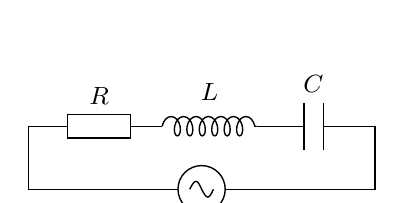
\begin{tikzpicture}[x=1cm,y=1cm,line width=0.5pt,>=Stealth,font=\small]
\draw (0,0)--(0.5,0); \draw[fill=white] (0.5,-0.15) rectangle (1.3,0.15); \node[above] at (0.9,0.15) {$R$};
\draw (1.3,0)--(1.7,0); \draw[decorate,decoration={coil,aspect=0.6,segment length=4.5,amplitude=3.5}] (1.7,0)--(2.9,0); \node[above] at (2.3,0.2) {$L$};
\draw (2.9,0)--(3.5,0); \draw (3.5,-0.3)--(3.5,0.3) (3.75,-0.3)--(3.75,0.3); \node[above] at (3.62,0.3) {$C$}; \draw (3.75,0)--(4.4,0);
\draw (0,0)--(0,-0.8)--(1.9,-0.8); \draw (2.5,-0.8)--(4.4,-0.8)--(4.4,0); \draw (2.2,-0.8) circle(0.3); \draw (2.05,-0.8) sin (2.13,-0.7) cos (2.2,-0.8) sin (2.28,-0.9) cos (2.35,-0.8);
\end{tikzpicture}\end{center}
\noindent\textbf{33.}\ Zanjirdagi tok kuçining effektiv qiymatini (A) toping.\par
\noindent\textbf{34.}\ Rezistordagi kuçlanişning effektiv qiymatini (V) toping.\par
\noindent\textbf{35.}\ Zanjirda ajralayotgan aktiv quvvatni (W) toping.\par
\noindent Variantlar: A) 1;\quad B) 2;\quad C) 60;\quad D) 100;\quad E) 120;\quad F) 200\par\smallskip
\noindent\colorbox{gray!12}{\parbox{\dimexpr\linewidth-2\fboxsep}{\textbf{Javob: 33--B) 2; 34--C) 60; 35--E) 120}}}\par\smallskip
\noindent\textit{Yechim.}\ Töla qarşilik\par
\[Z=\sqrt{R^2+(X_L-X_C)^2}=\sqrt{30^2+40^2}=50\ \Omega,\qquad I=\frac{U}{Z}=2\ \text{A}.\]
$U_R=IR=60$ V, aktiv quvvat $P=I^2R=4\cdot30=120$ W.\par\par\medskip\hrule\medskip
\Needspace{12\baselineskip}\noindent\textbf{36.}\ Suv osti kemasi dengizda 50 m çuqurlikda suzmoqda. Dengiz suvining ziçligi 1030 kg/m$^3$, atmosfera bosimi 100 kPa, $g=10$ m/s$^2$.\par
\noindent\hspace*{4mm}a)\ Şu çuqurlikdagi töliq bosimni (kPa) toping.\par
\noindent\hspace*{4mm}b)\ Yuzasi 0,5 m$^2$ bölgan lyukka suv tomonidan ta’sir qiluvçi töliq bosim kuçini (kN) toping.\par
\noindent\colorbox{gray!12}{\parbox{\dimexpr\linewidth-2\fboxsep}{\textbf{Javob: a)\ 615;\quad b)\ 307,5}}}\par\smallskip
\noindent\textit{Yechim.}\ $p=p_0+\rho gh=100+1030\cdot10\cdot50/1000=615$ kPa. $F=pS=615\cdot0{,}5=307{,}5$ kN.\par\par\medskip\hrule\medskip
\Needspace{12\baselineskip}\noindent\textbf{37.}\ Gorizontal sirtda 10 m/s tezlik bilan sirpana boşlagan jism işqalaniş tufayli töxtadi. Işqalaniş koeffitsiyenti 0,25, $g=10$ m/s$^2$.\par
\noindent\hspace*{4mm}a)\ Jismning töxtagunça bosib ötgan yölini (m) toping.\par
\noindent\hspace*{4mm}b)\ Jismning töxtagunça ketgan vaqtini (s) toping.\par
\noindent\colorbox{gray!12}{\parbox{\dimexpr\linewidth-2\fboxsep}{\textbf{Javob: a)\ 20;\quad b)\ 4}}}\par\smallskip
\noindent\textit{Yechim.}\ $a=\mu g=2{,}5$ m/s$^2$; $s=\frac{v^2}{2a}=\frac{100}{5}=20$ m; $t=\frac{v}{a}=4$ s.\par\par\medskip\hrule\medskip
\Needspace{12\baselineskip}\noindent\textbf{38.}\ Uzunligi 0,5 m bölgan ipga osilgan 0,2 kg massali şarça gorizontal tekislikda aylana çizib aylanmoqda (konussimon mayatnik). Ip vertikal bilan $37^\circ$ burçak hosil qiladi. $\sin37^\circ=0{,}6$, $\cos37^\circ=0{,}8$, $g=10$ m/s$^2$.\par
\noindent\hspace*{4mm}a)\ Ipning taranglik kuçini (N) toping.\par
\noindent\hspace*{4mm}b)\ Şarçaning çiziqli tezligini (m/s) toping.\par
\noindent\colorbox{gray!12}{\parbox{\dimexpr\linewidth-2\fboxsep}{\textbf{Javob: a)\ 2,5;\quad b)\ 1,5}}}\par\smallskip
\noindent\textit{Yechim.}\ Vertikal yönalişda $T\cos\alpha=mg$: $T=\frac{2}{0{,}8}=2{,}5$ N. Aylana radiusi $r=l\sin\alpha=0{,}3$ m, $\mathrm{tg}\,\alpha=\frac{v^2}{gr}$:\par
\[v=\sqrt{gr\,\mathrm{tg}\,\alpha}=\sqrt{10\cdot0{,}3\cdot0{,}75}=1{,}5\ \text{m/s}.\]\par\medskip\hrule\medskip
\Needspace{12\baselineskip}\noindent\textbf{39.}\ Gaz 200 kPa özgarmas bosimda 3 L dan 5 L gaça kengaydi. Gazning dastlabki temperaturasi 300 K.\par
\noindent\hspace*{4mm}a)\ Gazning bajargan işini (J) toping.\par
\noindent\hspace*{4mm}b)\ Gazning oxirgi temperaturasini (K) toping.\par
\noindent\colorbox{gray!12}{\parbox{\dimexpr\linewidth-2\fboxsep}{\textbf{Javob: a)\ 400;\quad b)\ 500}}}\par\smallskip
\noindent\textit{Yechim.}\ $A=p\Delta V=2\cdot10^5\cdot2\cdot10^{-3}=400$ J. Izobarik: $T_2=T_1V_2/V_1=300\cdot5/3=500$ K.\par\par\medskip\hrule\medskip
\Needspace{12\baselineskip}\noindent\textbf{40.}\ 3 kg suvni 20 $^\circ$C dan 70 $^\circ$C gaça isitiş uçun spirt yondirildi. Isitgiçning FIK 50\%. $c_{suv}=4200$ J/(kg$\cdot$K), $q_{spirt}=30$ MJ/kg.\par
\noindent\hspace*{4mm}a)\ Suv olgan issiqlik miqdorini (kJ) toping.\par
\noindent\hspace*{4mm}b)\ Yondirilgan spirt massasini (g) toping.\par
\noindent\colorbox{gray!12}{\parbox{\dimexpr\linewidth-2\fboxsep}{\textbf{Javob: a)\ 630;\quad b)\ 42}}}\par\smallskip
\noindent\textit{Yechim.}\ $Q=4200\cdot3\cdot50=630$ kJ. $\eta qm=Q$:\par
\[m=\frac{630\cdot10^3}{0{,}5\cdot30\cdot10^6}=0{,}042\ \text{kg}=42\ \text{g}.\]\par\medskip\hrule\medskip
\Needspace{12\baselineskip}\noindent\textbf{41.}\ Siğimi 2 $\mu$F bölgan yassi kondensator 100 V kuçlanişgaça zaryadlanib, manbadan uzildi. Söngra qoplamalar orasidagi masofa 2 marta orttirildi.\par
\noindent\hspace*{4mm}a)\ Kondensator qoplamalari orasidagi yangi kuçlanişni (V) toping.\par
\noindent\hspace*{4mm}b)\ Kondensatorning yangi energiyasini (mJ) toping.\par
\noindent\colorbox{gray!12}{\parbox{\dimexpr\linewidth-2\fboxsep}{\textbf{Javob: a)\ 200;\quad b)\ 20}}}\par\smallskip
\noindent\textit{Yechim.}\ Manbadan uzilgan — zaryad özgarmas: $q=CU=200\ \mu$C. Masofa 2 marta ortsa $C'=1\ \mu$F, $U'=200$ V.\par
\[W'=\frac{qU'}{2}=\frac{2\cdot10^{-4}\cdot200}{2}=0{,}02\ \text{J}=20\ \text{mJ}.\]\par\medskip\hrule\medskip
\Needspace{12\baselineskip}\noindent\textbf{42.}\ Radiusi 10 cm bölgan metall sferaga 2 nC zaryad berilgan. $k=9\cdot10^9$ N$\cdot$m$^2$/C$^2$.\par
\noindent\hspace*{4mm}a)\ Sfera markazidan 20 cm masofadagi maydon kuçlanganligini (V/m) toping.\par
\noindent\hspace*{4mm}b)\ Sfera markazidagi maydon potensialini (V) toping.\par
\noindent\colorbox{gray!12}{\parbox{\dimexpr\linewidth-2\fboxsep}{\textbf{Javob: a)\ 450;\quad b)\ 180}}}\par\smallskip
\noindent\textit{Yechim.}\ Sfera taşqarisida maydon nuqtaviy zaryadnikidek: $E=\frac{kq}{r^2}=\frac{9\cdot10^9\cdot2\cdot10^{-9}}{0{,}04}=450$ V/m. Sfera içida potensial sirtdagi bilan bir xil: $\varphi=\frac{kq}{R}=\frac{18}{0{,}1}=180$ V.\par\par\medskip\hrule\medskip
\Needspace{12\baselineskip}\noindent\textbf{43.}\ Metalldan elektronlarning çiqiş işi 2 eV. Metallga energiyasi 3,5 eV bölgan fotonlar tuşmoqda. $hc=1240$ eV$\cdot$nm.\par
\noindent\hspace*{4mm}a)\ Fotoelektronlarning maksimal kinetik energiyasini (eV) toping.\par
\noindent\hspace*{4mm}b)\ Şu metall uçun fotoeffektning qizil çegarasini (nm) toping.\par
\noindent\colorbox{gray!12}{\parbox{\dimexpr\linewidth-2\fboxsep}{\textbf{Javob: a)\ 1,5;\quad b)\ 620}}}\par\smallskip
\noindent\textit{Yechim.}\ $E_k=\varepsilon-A=3{,}5-2=1{,}5$ eV. $\lambda_{qiz}=\frac{hc}{A}=\frac{1240}{2}=620$ nm.\par\par\medskip\hrule\medskip
\Needspace{12\baselineskip}\noindent\textbf{44.}\ Sindiruvçi burçagi $6^\circ$ bölgan yupqa şişa prizmaga yoruğlik nuri kiçik burçak ostida tuşmoqda. $n_{shisha}=1{,}5$, $n_{suv}=4/3$.\par
\noindent\hspace*{4mm}a)\ Prizma havoda bölganda nurning oğiş burçagini (gradusda) toping.\par
\noindent\hspace*{4mm}b)\ Prizma suvga botirilganda nurning oğiş burçagini (gradusda) toping.\par
\noindent\colorbox{gray!12}{\parbox{\dimexpr\linewidth-2\fboxsep}{\textbf{Javob: a)\ 3;\quad b)\ 0,75}}}\par\smallskip
\noindent\textit{Yechim.}\ Yupqa prizmada oğiş burçagi $\delta=(n_{nis}-1)\varphi$. Havoda $\delta=0{,}5\cdot6^\circ=3^\circ$. Suvda $n_{nis}=1{,}5/(4/3)=1{,}125$, $\delta=0{,}125\cdot6^\circ=0{,}75^\circ$.\par\par\medskip\hrule\medskip
\Needspace{12\baselineskip}\noindent\textbf{45.}\ Radioaktiv namunadagi yadrolar soni 30 sutkada 8 marta kamaydi.\par
\noindent\hspace*{4mm}a)\ Izotopning yarim yemiriliş davrini (sutka) toping.\par
\noindent\hspace*{4mm}b)\ Yana neça sutkadan keyin yadrolar soni boşlanğiç sonning 1/32 qismiga teng böladi?\par
\noindent\colorbox{gray!12}{\parbox{\dimexpr\linewidth-2\fboxsep}{\textbf{Javob: a)\ 10;\quad b)\ 20}}}\par\smallskip
\noindent\textit{Yechim.}\ $8=2^3$ — 30 sutka 3 ta yarim yemiriliş davri, $T=10$ sutka. $1/32=2^{-5}$ — jami 50 sutka, ya’ni yana $50-30=20$ sutka.\par\par\medskip\hrule\medskip
\end{document}